\documentclass[manuscript.tex]{subfiles}
\begin{document}
\setcounter{chapter}{1}
\author{\and{Luke Thomas Smith} \and{Tom Horrocks} \and{Eun-Jung Holden} \and{Daniel Wedge} \and{Naveed Akhtar}}
\title{Physics-informed Implicit Neural Representation for Potential Field Geophysics}
\date{\today}
\maketitle{}

\begin{abstract}
    The recent use of spatial coordinate features in multilayer perceptron (MLP) neural networks provides opportunities for novel applications in potential field geophysics.
    So called coordinate MLP networks allow for implicit learning of potential field samples as a function of their recorded sample locations.
    Using this new paradigm of encoding spatial information within a neural network enables new methods for working with potential field survey data.
    We demonstrate the quality of the learnt implicit potential field function by encoding real airborne geophysical survey line data, and predicting constant level grids of arbitrary cell size.
    We further demonstrate the potential for processing the learnt function in the continuous domain using automatic differentiation, with the same framework used to train the neural network.
    For example, directional gradients and subsequent filters are calculated prior grid quantisation, and therefore without the associated loss of high-resolution content imposed by gridding.
    The training process requires only the sample coordinates and recorded potential field for a single survey extent, and can be applied to various geophysical techniqes including magnetics and gravity. %, as well as radiometric or other grids.
\end{abstract}

\section{Introduction}
Geophysical potential fields are continuous functions in three dimensions, and are of importance to geoscience and mineral exploration.
When surveying these fields for exploration geophysics, sample locations are scattered in x, y, and z, despite best efforts to conform to a regular grid or line sample structure.
These scattered data are typically regularised to a quantised grid, which reduces high frequency information and gives rise to spurious artefacts that are a product of the gridding process, not the surveyed field.
If a representation of the potential field could instead be encoded within a neural network, it is possible that high frequency information would be preserved in a continuous domain.
Within the continuous representation, grid resolution is not constrained by an initial cell size selection, and further processing and filters can be calculated analytically in the continuous spatial domain.
This allows the use of all available sample information in the calculation of filters, and reduces the manual intervention required during the gridding process.

Encoding a potential field into a neural network can be performed using the recent technique of implicit neural representation.
Implicit neural representation (INR) is the task of representing a signal as a function of its coordinates.
Networks designed to learn such functions are known as coordinate multilayer perceptrons, or coordinate MLPs.
By parameterising the neural function in coordinate space, novel values of the function can be queried at arbitrary coordinates within the learnt continuous spatial domain.
Coordinate MLPs have recently benefit from high frequency representation improvements through the use of periodic activations.
Periodic activations such as sinusoids are continuously differentiable through the depth of the network, supporting high quality learning of implicit functions.

Furthermore, these cordinate MLP networks can be constrained to obey geophysical laws, using physics-informed neural network regularisation.
Imposing restrictions such as Laplace's equation on the network reduces the model search space, stabilising and speeding up training and predicting solutions that obey these laws.

The proposed method leverages recent approaches in the literature to learn a continuous volume of potential field geophysics, using a novel combination of physics-informed networks and implicit neural representation.
This implicit representation is used to generate levelled 2D grids directly from scattered sample data, as well as calculate gradients and further filters.
These are compared against industry standard gridding methods and numerical filters.

\subsection{Geophysical sampling and regularisation}
\label{sec:geo_airborne}
Airborne or ground-based potential field surveys sample a magnetic (or gravitational) scalar field on a three-dimensional drape surface.
Cultural obstructions or topography within the survey extent cause this drape surface to be irregular, and the sample points scattered.
The resolvable detail within the sampled field is a function of the sampling density, and the distance from the source.
% It is common to define a nominally regular drape surface with these parameters in mind, while respecting the cost of acquisition.
To enable digital processing and storage of the sample data following acquisition, the scattered points are regularised to a quantised grid.
The Nyquist wavelength inherent to the selected grid cell size during regularisation limits the high-resolution information representable by the grid.
Because grid regularisation is one of the earliest steps in interpreting geophysical surveys, this information fails to be utilised in most tasks.
% Subsequent processes such as frequency filtering or directional gradients are similary constrained by the parameters of the regularisation.
% Additionally, storing the grid product requires amount of memory, to represent the value with adequate precision at each cell in the resulting grid.

\label{sec:geo_physics}
Magnetic and gravitational fields in geophysics are conservative vector fields, but are typically sampled as a scalar potential field in a single direction.
Representing a vector field requires three orthogonal components at each spatial coordinate, while a scalar field can be parameterised with a single component \parencite{blakelyPotentialTheoryGravity1996}.
A potential field survey can be parameterised as
\begin{equation}
    u = \phi\left(x,y,z\right)
\end{equation}


Potential fields in an airborne sampling context are constrained by a number of physical laws, including \emph{Laplace's equation},
\[
    \nabla^2 \phi = 0
\]
In three dimensions \( \phi\left(x,y,z\right) \):
\begin{equation}
    \label{eqn:Laplace}
    \frac{\partial{}^2\phi}{\partial{}x^2} + \frac{\partial{}^2\phi}{\partial{}y^2} + \frac{\partial{}^2\phi}{\partial{}z^2} = 0
\end{equation}
%TODO Confirm logic here: % If Laplace's equation:\( \nabla^2 \phi = 0 \) is satisfied, it is harmonic, and has continuous single valued first derivatives, and has second derivatives.
% This indicates the function lacks curvature. 

% Blakely:
% A force field \(F\) is the gradient (or negative gradient) of the potential energy.
% \( F = \nabla\phi \) for the gravity potential, \(F = - \nabla \phi\) for the Magnetic potential.
% \( \phi(x,y,z) = constant \) is an equipotential surface.

% Numerical methods for potential field continuation are unstable, recognised in the geophysical community by solution divergence and noise in predictions.

\subsection{Implicit neural representation}
\label{sec:inr}
Multilayer perceptron (MLP) networks are fully connected networks, which have been ubiquitous in machine learning for several decades.
An MLP comprises a sequence of layers of neurons, densely connected to all neurons in each adjacent layer.
Each neuron is a discrete trainable function, comprising a weight multiplied by the input vector, an added bias term, and a subsequent scaling function termed the activation function.
The structure of an MLP can be described by the number of neurons in each layer (features) the number of layers between the input and output (hidden layers), and the class of activation function used.

A classic example MLP is an input vector of image pixel intensities \(u\), and an output vector of class labels \(l\). %, scaled by a function that transforms the output to a class probability.
Training this example network with a large number of different images with class labels produces a model capable of predicting the class of novel input image vectors.
A Coordinate MLP (CMLP) instead takes an input of explicitly stated pixel coordinates \((x,y)\), and an output vector of image pixel intensities \(u\) at those coordinates.
Training the CMLP requires a set of input coordinates and intensities from a single image, and results in a model capable of predicting the intensity of any arbitrary continuous coordinate within the input domain.
Both tasks may use similar images and an MLP network structure with the same \(n\) hidden layers and \(m\) hidden features, but the use of coordinates as inputs and intensities as outputs changes the predictive task.
Coordinate MLP networks for predicting scalar fields are a class of neural networks \(f\) which train \(u = f(x,y,z)\), with \(u\in\mathbb{R}^1\) and \((x,y,z)\in\mathbb{R}^3\).

Seminal work by \parencite{mildenhallNeRFRepresentingScenes2020} demonstrated implicit neural representation of volume density and colour dimensions, learnt from five dimensions of radiance and spatial coordinates.
However, it was not until the use of periodic activation functions such as the sinusoid \parencite{sitzmann2019siren} that implicit representation with CMLP networks could adequately recreate high frequency signals.
Periodic activation functions differ from non-linear activations such as ReLU by comprising the neuron with a function which repeats periodically, which allows for continuous differentiation throughout the depth of the network.
Work by \parencite{ramasinghePeriodicityUnifyingFramework2022} revealed that it is the magnitude of the first and second derivatives of the activation that enhance high-frequency capacity, rather than periodicity, leading to Gaussian \parencite{ramasinghePeriodicityUnifyingFramework2022} and wavelet \parencite{saragadamWIREWaveletImplicit2023} activation functions for CMLP\@.
%TODO Confirm re: blakely % ReLU has constant second derivative of zero, rendering it incapable of representing a harmonic function such as a potential field.

Coordinate MLPs can be used for a variety of computer vision tasks, including three-dimensional point cloud representation \parencite{qiPointNetDeepHierarchical2017}, and two-dimensional natural image representation tasks such as super-resolution and infilling \parencite{leeLocalTextureEstimator2022,chenLearningContinuousImage2021}.
Resolution in these tasks is not limited by quantisation of the representation, but rather the capacity of the network architecture used.
Increasing this capacity is currently the subject of very high interest in the machine learning research community, for example by leveraging new activation functions \parencite{saragadamWIREWaveletImplicit2023}, transforming the input space \parencite[e.g.][]{benbarkaSeeingImplicitNeural2022}, or using additional constraints on the search space such as physics-informed neural networks \parencite{raissiPhysicsinformedNeuralNetworks2019}.

\subsection{Physics-informed neural networks}
\label{sec:pinn}
Physics-informed neural networks (PINNs) recognise that if the inputs to a neural network are samples of a function which follows some physical law, outputs from the model should similarly be constrained by that law.
By regularising the network with an objective function which penalises solutions that don't fit the partial differential equations describing the law, it is possible to vastly reduce the physically valid solution search space.
Examples of physics-informed constraints include enforcing initial or boundary conditions, or adherence to known properties of the modelled signal.
As described in \cref{sec:geo_physics}, potential fields in geophysics obey \emph{Laplace's equation}, that the sum of partial second derivates is 0.
Because CMLP networks with periodic activations are continuously differentiable, it is possible to enforce this constrain as an element of the overall loss function within the network.
In addition to \(L^2\) (Mean Square Error) loss between the input and predicted coordinate values, a geophysics informed network could include a Laplace criterion \cref*{eqn:cri_laplace}.

\begin{equation}
    \label{eqn:cri_laplace}
    \mathcal{L}_{PDE} = \beta{}\lVert{}\frac{\partial{}^2\phi}{\partial{}x^2} + \frac{\partial{}^2\phi}{\partial{}y^2} + \frac{\partial{}^2\phi}{\partial{}z^2}\rVert{}_{2}
\end{equation}

As denoted by the \(L^2\) operator \(\lVert{}\cdot{}\rVert{}_{2}\) and weighting \(\beta{}\), this criterion penalises predictions that are not close to zero.

\Textcite{sethiHardEnforcementPhysicsinformed2023} demonstrate that this regularisation does not have to be implemented as a loss function, but instead can be a hard constraint embedded within the network.
This hard constraint takes the form of a function, which satisfies the \emph{a priori} laws, applied to the output of the network prior PDE and regularisation.
Another approach \parencite{liImplicitStochasticGradient2023} replaces the ubiquitous stochastic gradient descent optimiser \emph{Adam} with an implicit stochastic gradient descent (ISGD) method.
However, only the approach of \textcite{benbarkaSeeingImplicitNeural2022} is implemented for this work.
% This method reduces the importance of batch size and learning rate
% \[\theta_{n+1} = \theta_{n} - \alpha \cdot \nabla L (\theta_{n+1})\]

\subsection{Automatic Differentiation}
Automatic differentiation (AD) refers to one of several methods for computing derivatives, specifically to the accumulation of derivatives during function evaluation \parencite{baydin2018automatic}.
This method underpins modern machine learning frameworks such as Pytorch \parencite{paszkePyTorchImperativeStyle2019}, which the framework used to construct the network architecture and perform training in this work.
In these frameworks, training is performed by evaluating the result of a set of inputs using the current model weight parameters during a forward pass, accumulating the partial derivatives with respect to the parameters, and minimising an objective (loss) function using those gradients.
These gradients inform weight updates in the direction of the negative gradient, toward a minima in the objective function.
However, automatic differentiation can also evaluate the derivatives with respect to the inputs, using the same high-performance AD framework (e.g. Pytorch).
This can provide the partial derivatives \(\frac{\partial f}{\partial x}, \frac{\partial f}{\partial y}, \frac{\partial f}{\partial z}\), as well as higher order derivatives.

\section{Method}
% \subsection{Notation}
% Real n-dimensional vectors, named using lower-case letters are noted \(\mathbb{R}^n\), e.g. \boldmath{u}.
% \(\mathbb{R}^{m\times{}n}\) \(m*n\) dimensional matrices, named using upper-case letters, e.g. \boldmath{A}.

\subsection{Data}
A case study dataset is made using the 2002 Wolfe Creek meteorite impact magnetic survey (Geophysical Acquisition \& Processing Section \cite*{wolfecreek2019}).
This high-resolution survey contains \SI{402}{line-kilometres} of data at \SI{50}{\m} line spacing with a nominal terrain clearance of \SI{40}{\m}.
The data used for implicit representation include the survey tie lines, standard in airborne geophysical surveys to reduce inter-line levelling noise.
The standard deviation of the drape surface, including tie lines, is \SI{5}{\m}.

Both the line data netCDF and grid raster for the Wolfe Creek survey were downloaded from the Geoscience Australia Geophysical Archive Data Delivery System and used without further processing.
The line data netCDF contains tie-levelled, micro-levelled, and AWAGS levelled magnetic variables, in respective order of processing levels.
% Tie-levelling is applied using only line data, while micro-levelling uses parameters calculated on an intermediate grid product of the line data.
% AWAGS levelling is a final continuation of the microlevelled dataset to an Australian common datum, termed the \emph{AWAGS} datum.
For the Wolfe Creek survey, the microlevelled magnetic data are used.
Both geographic and projected coordinate systems can be used, provided the query coordinates for inference match those used during training.
The three spatial coordinate dimensions are independently linearly min-max normalised between -1 and 1.
While this means the latent spatial domain may be compressed relative to each other axis, the inverse normalisation process returns proportionality between axes.
The case study data do not span a large or magnetically varying geological extent, hence it is sufficient to use simple min-max normalisation for the magnetic field data within the global extent of the survey samples, here between -1 and 1.
If extensive or complexly varying magnetic provinces were present within the dataset, a normalisation method more robust to outliers may be required.

In order to validate the model performance during training, a random \qty{20}{\percent} of the survey sample points are reserved.
% Not currently doing this % Testing of the model is performed on a randomly selected \qty{10}{\percent} of the sample points. 
Inference can be performed by querying novel coordinates within the learnt domain, here at regularly spaced grid intervals for comparison with standard grid regularisation methods.

\subsection{Network architecture}
The Coordinate MLP architecture comprises a simple fully connected network with \(N\) hidden layers, each with \(m\) neurons.
The sinusoidal activation of \cite{sitzmann2019siren} is used. % for a baseline, and comparison is made to Gaussian and wavelet activations.
High quality implicit representation has been achieved in contemporary INR research with only several hidden layers, typically between 3 and 8, with \(N = 8\) is used here.
The number of neurons per layer is set \(m = 256\).
% Figure \cref{fig:arch} shows the structure of the architecture.

% \begin{figure}[hbt]
%     \label{fig:arch}
%     \caption[Network Architecture]{The Coordinate MLP architecture used for the implicit neural representation task.}
% \end{figure}

\subsection{Training Particulars}
\label{sec:training}
% Performed on an Intel i5-12400 CPU with 32 GB RAM, and an Nvidia 3060 12 GB GPU.

Implicit functions are trained using coordinate-value pairs, and for low-resolution images the entire cell coordinate and cell value dataset fits within GPU memory for batch gradient descent.
The Wolfe Creek meteorite impact crater case study line data has \SI{76420}{} sample points, with the Geoscience Australia provided grid product having a resolution of 446 \(\times{}\) 445 cells.
The line coordinate dataset easily fits into available graphics memory, and can be trained using batch gradient descent.
%However, training on large scattered aeromagnetic surveys with more than one million samples, memory becomes a constraint and mini-batch training is required.
Training was performed on an Intel i9-10900KF workstation with an Nvidia RTX 3090 24 GB GPU\@.
A highly accurate representation can be learned within 1000 epochs using the Adam optimiser, for a duration in the order of 60 seconds.
The OneCycle learning rate scheduler \parencite{smithSuperconvergenceVeryFast2018} with a maximum rate of \(3\times{}10^{-4}\) is used to provide fine tuning at low learning rates toward the end of training.
Convergence of the network is shown in \cref{fig:convergence}

\begin{figure}[hbt]
    \centering{}
    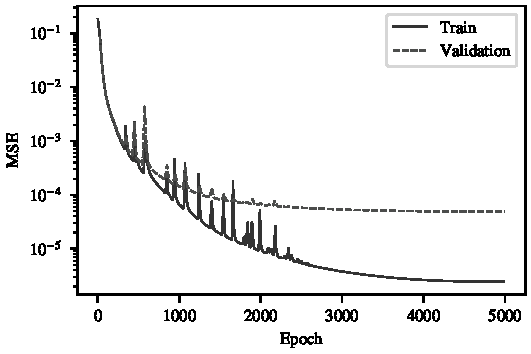
\includegraphics[width=0.5\linewidth]{fig/p3/loss_plot.pdf}
    \caption[Training convergence]{Train and validation loss for the duration of the experiment.}
    \label{fig:convergence}
\end{figure}

As described in \cref{sec:pinn}, the objective function comprises \(L^2\) loss between the input and predicted field values.
It does not use the Laplace loss discussed in \cref{sec:pinn}, which fails to converge. %, summed with weighted Laplace's equation loss, \cref{eqn:cri}.
\begin{equation}
    \label{eqn:cri}
    \mathcal{L}_{Total} = \lVert{}u_{input} - u_{pred}\rVert{}_{2} % + \beta{} \lVert{}\frac{\partial^{2}{u_{pred}}}{\partial{}\phi{}_{pred}^{2}}\rVert{}_{2}
\end{equation}

\subsection{Derivative calculation}
A naive approach to calculating gradients with the INR would be to evaluate the representation \(\phi{}_{(x, y, z)}\) at a set of regular coordinates \({(x, y, z)}_1 \dots {(x,y,z)}_n\), and use numerical differentiation to calculate derivatives.
However, using Automatic Differentiation with Pytorch, the implicit representation can be differentiated with respect to its inputs to provide gradients, prior to being queried at the nodes of a quantised grid.
That is, directly sample \(\nabla{}\phi{}_{(x,y,z)}\) at \({(x, y, z)}_1 \dots {(x,y,z)}_n\).
Higher order derivatives can be also calculated using AD in this manner.

\section{Results}
\subsection{Implicit gridding}
Querying a learnt implicit neural representation (INR) using a regularly spaced \(x,y\) grid at a specific \(z\) height is a novel method for gridding geophysical potential field surveys.
\Cref{fig:grid} shows the INR queried at \(z=\SI{40}{\meter}\), which is the nominal terrain clearance of the survey.
Notably, the cell size can be selected by fining or coarsening the \(x,y\) spacing, including variable or anisotropic cell sizes.
Contemporary super-resolution research can leverage this continual representation as a framework for high quality arbitrary scale factor high-frequency component prediciton \parencite[e.g][]{chenLearningContinuousImage2021}.
However, the potential field representation task here does not attempt to predict additional high-frequency information and resolution remains limited by the survey sample spacing and neural network capacity.

\begin{figure}[hbt]
    \centering{}
    \includegraphics[width=1.0\linewidth]{fig/p3/grid_comparison_40m.pdf}
    \caption[Grid prediction]{Comparison between the ground-truth grid processed by Geoscience Australia (left) and the constant level grid queried from the INR at \SI{40}{\m} (right).}
    \label{fig:grid}
\end{figure}

The INR can be queried at any continuous coordinate, including out-of-range values beyond the training domain.
The predicted field becomes unstable beyond this boundary, which can be seen in the periphery of \cref{fig:grid}.

Constant level grids can be queried from the INR at any height.
\Cref{fig:grid35} shows the case study extent queried at \SI{35}{\m}.
While comparable features can still be interpreted within this level grid, the representation learnt here fails to represent physically realistic continuation of the field.
It is conjectured that implementing a PINN criterion such as Laplacian loss \cref{eqn:cri_laplace} would improve the performance these upward or downward extracted slices.

\begin{figure}[hbt]
    \centering{}
    % TODO query at AWAGS height and compare GA AWAGS grid.
    % TODO check if provided grid is AWAGS or MICRO levelled - maybe grid data myself.
    \includegraphics[width=1.0\linewidth]{fig/p3/grid_comparison_35m.pdf}
    \caption[Grid prediction]{A constant level grid queried from the INR at the height of \SI{35}{\m} (right).}
    % AWAGS is 80 m, but we see nothing useful at 80m
    \label{fig:grid35}
\end{figure}

% The strong performance of the model is retained even when using a subsampled training dataset, here shown at \qty{30}{\percent} and \qty{10}{\percent} (\cref{fig:gridpct}) of the total available data.
% % In both cases, the validaiton and test sets remain identical to the initial training split.

% \begin{figure}[hbt]
%     % \includegraphics[]{fig/p3/grid_subpct.pdf}
%     \caption[Grid subsampled]{Performance of level grid prediction shown at \qty{30}{\percent} and \qty{10}{\percent} random sampling of training data.}
%     \label{fig:gridpct}
% \end{figure}


\subsection{Spatial derivatives and filters}
Using AD, derivatives can be calculated between the input spatial coordinates and the output potential field representation.
While horizontal derivatives queried from the INR correspond well to numerical derivatives calculated on the 40 m level grid (\cref{fig:hori_grad}), the vertical derivative suffers poor performance (\cref{fig:vert_grad}).
This correlates with the poor continuation performance of model when predicting level grids several meters or more beyond the nominal sample height.
This is interpreted as the model learning a poor representation of the vertical component of the potential field.

\begin{figure}[hbt]
    \centering{}
    \includegraphics[width=1.0\linewidth]{fig/p3/dh_comparison.pdf}
    \caption[Horizontal derivatives]{AD (left column) and numerical (middle column) horizontal derivatives of the INR\@. Residuals are shown in the right column.}
    \label{fig:hori_grad}
\end{figure}

\begin{figure}[hbt]
    \centering{}
    \includegraphics[width=1.0\linewidth]{fig/p3/dv_comparison.pdf}
    \caption[Vertical derivative]{AD (left) and numerical (right) vertical derivatives of the INR\@.}
    \label{fig:vert_grad}
\end{figure}

% Using the implicit representation, a selection of common geophysical filters are calculated prior to quantisation.

% \begin{enumerate}
%     \item ASIG
%     \item tilt?
%     \item idk?
% \end{enumerate}


\section{Discussion}
The implicit representation has strong representative capacity for the horizontal components of the potential field, allowing extraction of level grids which are accurate against the ground truth grid.
Level grids can be generated at any height, with best performance achieved near the realised nominal survey altitude.
Performance worsens within approximately one standard deviation from that height (\SI{35} to \SI{45}{\m}), with gradual failure of the model outisde of that height range.
% Even when using a small subset of the dataset, this performance is retained.
It is interpreted from the poor quality of the vertical gradients and out-of-range predictions that the model is relying on learning a function between horizontally coplanar points, as opposed to a realistic vertical continuation function.
While quantised grids can be queried at any cell size, short wavelength information beyond the Nyquist limit of the survey line sampling is not predicted.
% TODO The addition of a PINN term for objective function ...

% The case study survey presented is very small compared to typical regional aeromagnetic surveys.
% A demonstration of the method on a large aeromagnetic survey, requiring minibatch training, is included in \cref{app:menzies}.
% Training of this representation follows the parameters outlined in \cref{sec:training}, which were optimised for the Wolfe Creek case study, with the addition of a shuffled minibatch size of \SI{1024000}\@.
% Attempts to train the CMLP with small batch sizes did not converge.%, reflecting the non-convergence result found for training on very large subsampling factors of the line dataset.

Implicit neural representation is a rapidly evolving field of research, and draws on contemporary deep learning improvements within related fields.
In addition to improving the high-frequency learning capacity, physics informed loss functions may allow higher quality vertical continuation performance.
The current method could trivially include additional target dimensions, which would allow representation learning of vector fields \(\mathbb{R}^{3}\) in three dimensions \(\mathbb{R}^{3}\).
This has potential application in tensor fields and associated predictive tasks, and these remain for future work.

\section{Conclusions}
High-resolution implicit neural representation of potential field geophysics surveys is achieved with the use of coordinate MLP neural networks.
Resolution in the representation is limited by network capacity, rather than initial grid cell size selection during regularisation.
Level grids can be extracted from these representations, emerging as a novel method for regularising scatter geophysical sample data.
Gradients and spatial filters can be caluclated using the full resolution of the learnt representation, and gridded \emph{a posteri} of gradient or filter calculation.


\section{Acknowledgements}
This project is funded by a Rio Tinto Iron Ore PhD scholarship.

\printbibliography{}

% \section{Appendix A}
% \label{app:menzies} %TODO format as "Appendix"
% The Menzies South ... Pxxxx survey contains xxx sample points across yyyy line kilometres, and was flown at a nominal terrain clearance of zz m.
% While a high-quality result is attainable using batch gradient descent on a subset of the survey points, minibatch gradient descent is demonstrated for the CMLP used to learn the full survey INR\@.


% \begin{figure}[hbt]
%     % \includegraphics[width=\textwidth]{fig/p3/menzies.pdf}
%     \caption[Menzies INR]{Level grid representation using minibatch gradient descent.}
%     \label{fig:vert_grad}
% \end{figure}

\end{document}